\chapter{Data}
\label{cha:data}

\section{Data acquisition}
\label{sec:data-acquisition}

The data was acquired at the \acrfull{sas} laboratory at Linköping University. The experiment --- as shown on Figure~\ref{fig:experimental-setup} --- consisted of exposing different gas combinations to the \acrshort{sicfet} sensor under a certain frequency cycle and recording its response, measured in \acrfull{ma}. The is then used to extract secondary features, namely average and slope values from certain regions of the frequency cycle.

\begin{figure}[!htb]
	\centering
	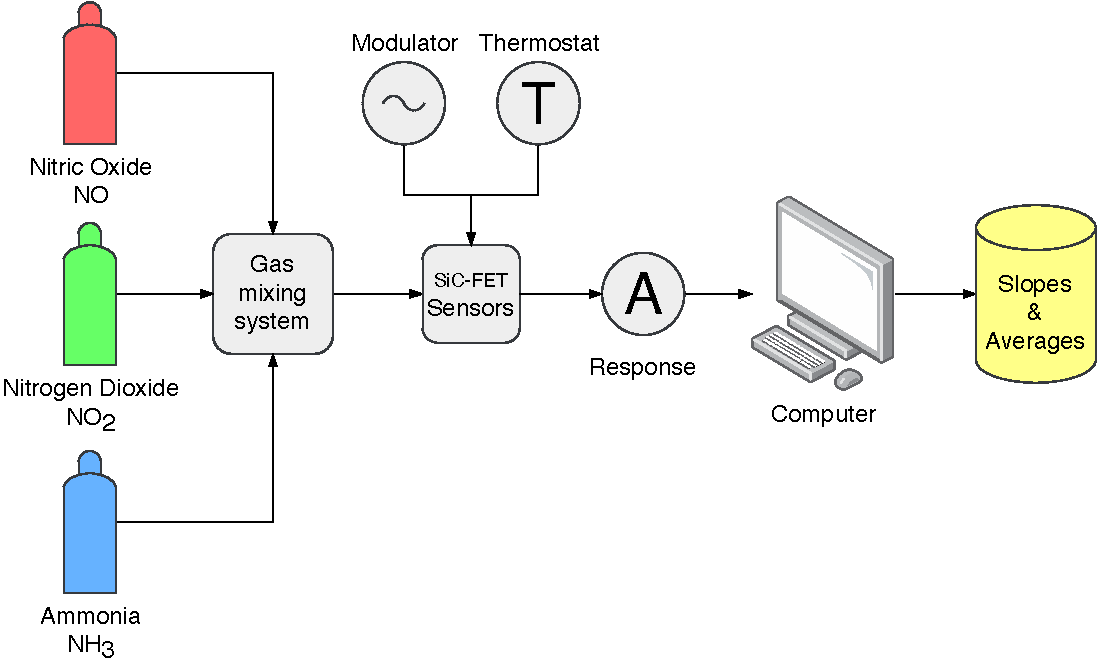
\includegraphics[width=0.8\textwidth]{../figures/experimental-setup.pdf}
	\caption{Schema of the data acquisition process.}
	\label{fig:experimental-setup}
\end{figure}

In more detail, \ch{NO}, \ch{NO2} and \ch{NH3} had five possible concentration values each: 10, 20, 40, 80 and 160 \acrfull{ppm}. The experiment was designed to encompass all possible combinations of these gasses, which totals to 125 different gas mixtures. Each feature was submitted to the same frequency cycle five times. The cycle consists of 16 unique frequencies: 0.05, 0.1, 0.25, 0.5, 1, 2, 5, 10, 25, 50, 100, 200, 500, 1000, 2500 and 5000 \acrfull{hertz}. A typical raw sensor response for frequency modulation experiments is shown on Figure~\ref{fig:raw}.

\begin{figure}[!htb]
	\centering
	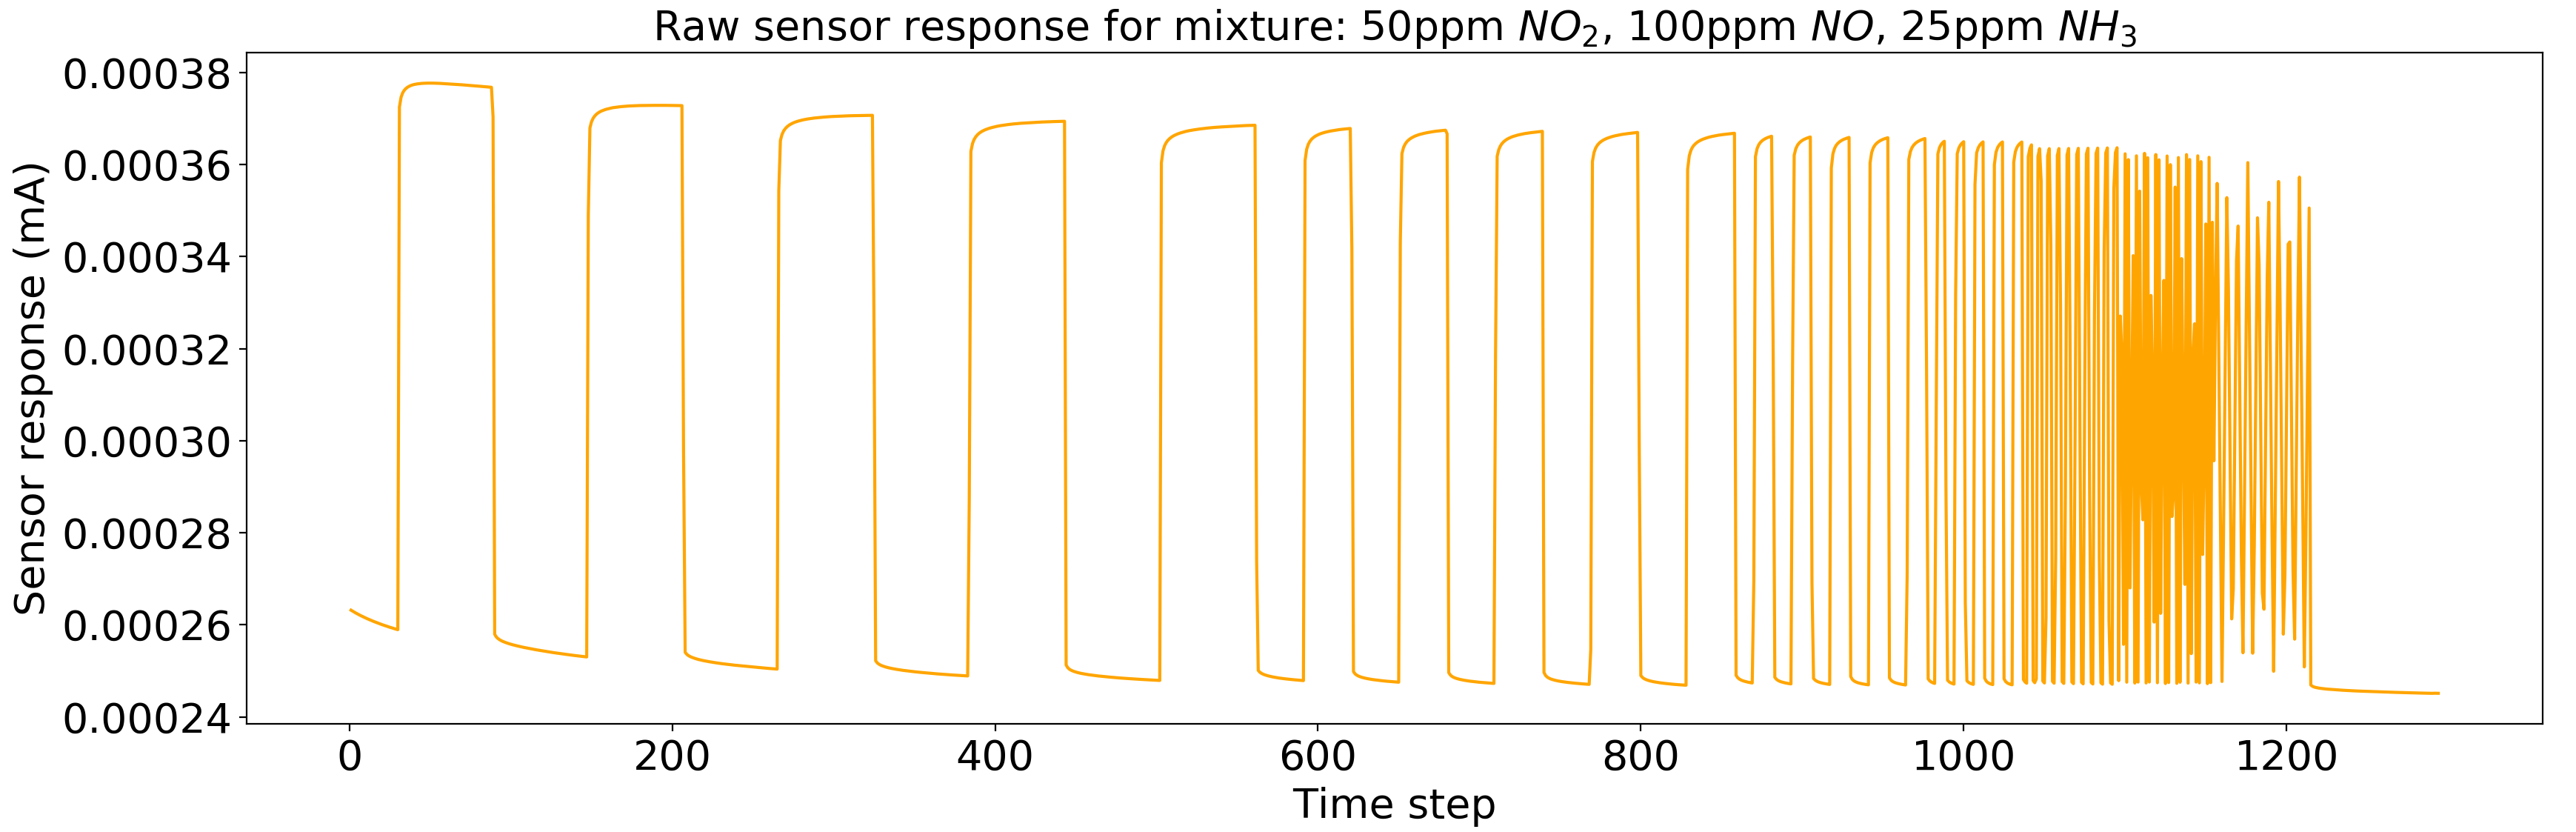
\includegraphics[width=1\textwidth]{../figures/raw-response.png}
	\caption{An example of row sensor response}
	\label{fig:raw}
\end{figure}

For each frequency in each cycle, two slope and two average features were extracted. These measurements were taken during a 0.4 second window, alternating between slope and average as shown on Figure~\ref{fig:feat-window}. Note that the y-axis of Figure~\ref{fig:feat-window} is in log-scale due to the different orders of magnitude that frequency achieves. Moreover, Figure~\ref{fig:experiment} gives more insight into feature measurement.

\begin{figure}[!htb]
	\centering
	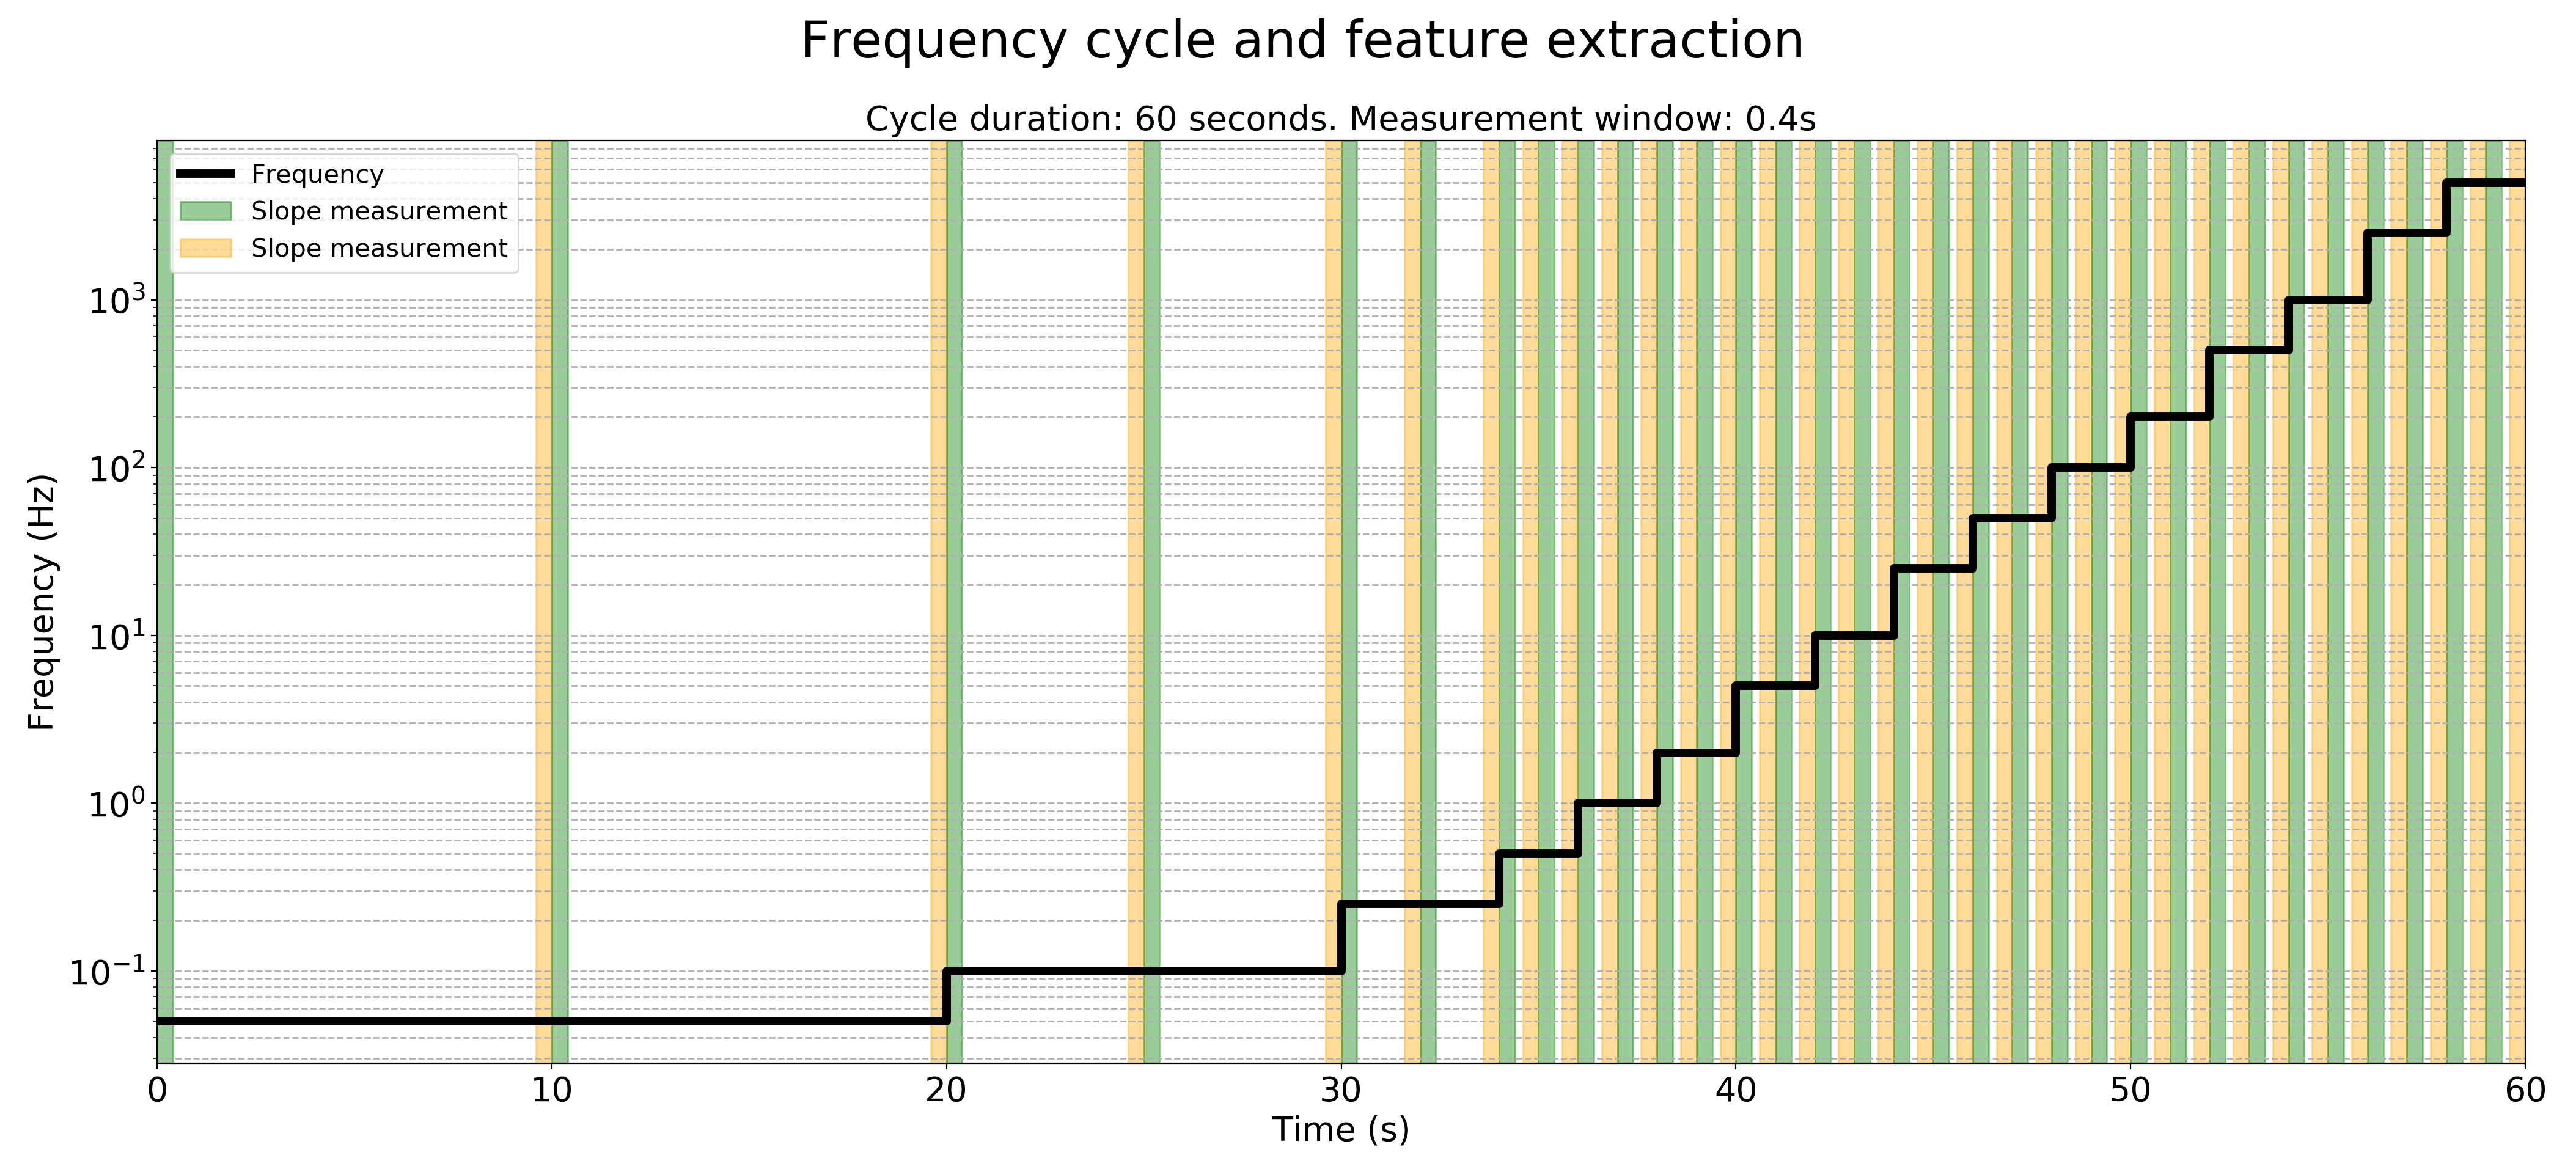
\includegraphics[width=1\textwidth]{../figures/measurement-windows.png}
	
	\caption{Feature measurements times per cycle.}
	\label{fig:feat-window}
\end{figure} 

\begin{figure}[h]
	\centering
	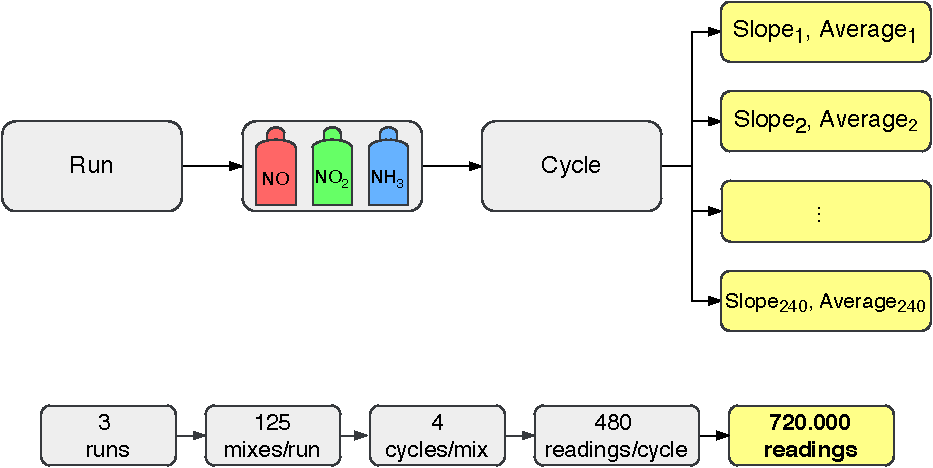
\includegraphics[width=0.8\textwidth]{../figures/features.pdf}
	\caption{A visualization of the feature measurement process for each gas mixture in each frequency cycle}
	\label{fig:experiment}
\end{figure}

Finally, all 125 gas mixtures were subjected to the experiment three times, each time at a different temperature as shown on Figure~\ref{fig:temps}. Table~\ref{tab:measurements} summarizes the data acquisition details.

\begin{figure}[!htb]
	\centering
	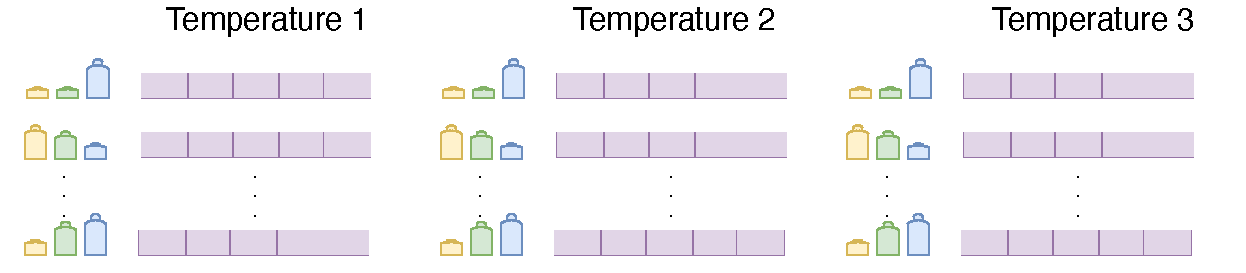
\includegraphics[width=1\textwidth]{../figures/temps.pdf}
	\caption{The same experiment was run with the sensor set to three different constant temperatures.}
	\label{fig:temps}
\end{figure}

\begin{table}[h]
	\centering
	\caption{Data acquisition details}
	\label{tab:measurements}
	\begin{tabular}{|c|c|}
		\hline
		\textbf{Parameter} & \textbf{Value} \\
		\hline
		Factors (gases) & 3 \\
		\hline
		Levels (concentrations) & 5 \\
		\hline
		Frequencies & 16 \\
		\hline
		Features per frequency & 4 (2 slopes and 2 averages) \\
		\hline
		Features per cycle & 64 \\
		\hline
		Number of cycles & 5 \\
		\hline
		Data points per mixture & 320 \\
		\hline
		Number of mixtures & 125 \\
		\hline
		Datapoints per experiment & 40.000 \\
		\hline
		Number of experiments & 3 \\
		\hline
		Total data points & 120.000 \\
		\hline
	\end{tabular}
\end{table}

For specific timestamps and measurement durations, the reader is referred to Appendix~\ref{app:A}.

\section{Raw data}
\label{sec:raw-data}

\section{Secondary data}
\label{sec:secondary-data}
